%%%%%%%%%%%%%%%%%%%%%%%%
%
% $Autor: Hemanth Jadiswami Prabhakaran $
% $Datum: 2025-06-29 19:44:08Z $
% $Pfad: GitHub/BA25-01-Time-Series/report/Contents/en/streamlit.tex $
% $Version: 1 $
%
% $Project: BA25-Time-Series $
%
%%%%%%%%%%%%%%%%%%%%%%%%


%
% !TeX encoding = utf8
% !TeX root = PythonPackages
%
%%%%%%%%%%%%%%%%%%%%%%%%

\chapter{Streamlit}
\label{ch:streamlit}

\section{Introduction}
\label{sec:intro}

Streamlit represents a revolutionary approach to building web applications for data science and machine learning projects \cite{Streamlit:2024}. Created by Adrien Treuille, Thiago Teixeira, and Amanda Kelly in 2019, Streamlit transforms Python scripts into interactive web applications with minimal code changes. The framework has gained significant traction in the data science community, enabling rapid prototyping and deployment of machine learning models without traditional web development complexity \cite{Chen:2023}. This chapter explores Streamlit's capabilities, providing comprehensive coverage of its features, implementation strategies, and practical applications for creating data-driven web applications.\\

The significance of Streamlit in the data application landscape stems from its simplicity and power. Traditional web development for data science applications required knowledge of HTML, CSS, JavaScript, and backend frameworks. Streamlit eliminates this barrier by providing a pure Python interface for creating interactive web applications \cite{Streamlit:2024}. Modern data science workflows benefit from Streamlit's ability to quickly transform Jupyter notebooks and Python scripts into shareable web applications, facilitating collaboration and stakeholder engagement \cite{Towards:2023}. The framework's integration with popular data science libraries like pandas, matplotlib, and scikit-learn has democratized web application development for data scientists and analysts.\\

\section{Description}
\label{sec:description}

\subsection{Core Capabilities}
\label{subsec:capabilities}

Streamlit offers a comprehensive suite of web application development capabilities:

\begin{itemize}
	\item \textbf{Rapid Development}: Transform Python scripts into web apps with minimal code changes
	\item \textbf{Interactive Widgets}: Built-in widgets for user input (sliders, buttons, file uploads)
	\item \textbf{Data Visualization}: Native support for matplotlib, plotly, altair, and custom charts
	\item \textbf{Machine Learning Integration}: Seamless deployment of ML models and predictions
	\item \textbf{Responsive Design}: Automatic mobile-friendly layouts and responsive components
\end{itemize}

\subsection{Python Framework: streamlit}
\label{subsec:streamlit}

The \texttt{streamlit} package provides a declarative approach to web application development. It offers intuitive functions for creating interactive elements:

\begin{lstlisting}[language=MyPython, caption={Streamlit Core Functions}, label={lst:streamlit_core}]
	
	import streamlit as st
	import pandas as pd
	
	# Display text and data
	st.title("My Streamlit App")
	st.write("Hello, World!")
	st.dataframe(df)
	
	# Interactive widgets
	name = st.text_input("Enter your name")
	age = st.slider("Select your age", 0, 100, 25)
	
	# Display results
	st.write(f"Hello {name}, you are {age} years old!")
	
\end{lstlisting}

\subsection{Use Cases}
\label{subsec:usecases}

Streamlit finds applications across diverse domains:

\begin{enumerate}
	\item \textbf{Data Dashboards}: Interactive visualization of business metrics and KPIs
	\item \textbf{Machine Learning Demos}: Rapid deployment of ML models for stakeholder review
	\item \textbf{Prototype Applications}: Quick development of proof-of-concept applications
	\item \textbf{Data Analysis Tools}: Interactive exploratory data analysis interfaces
	\item \textbf{Educational Tools}: Creating interactive learning materials and tutorials
\end{enumerate}

\subsection{Architecture Overview}
\label{subsec:architecture}

\begin{figure}[H]
	\centering
	% Streamlit Application Architecture TikZ Diagram
% File: streamlit_architecture.tikz

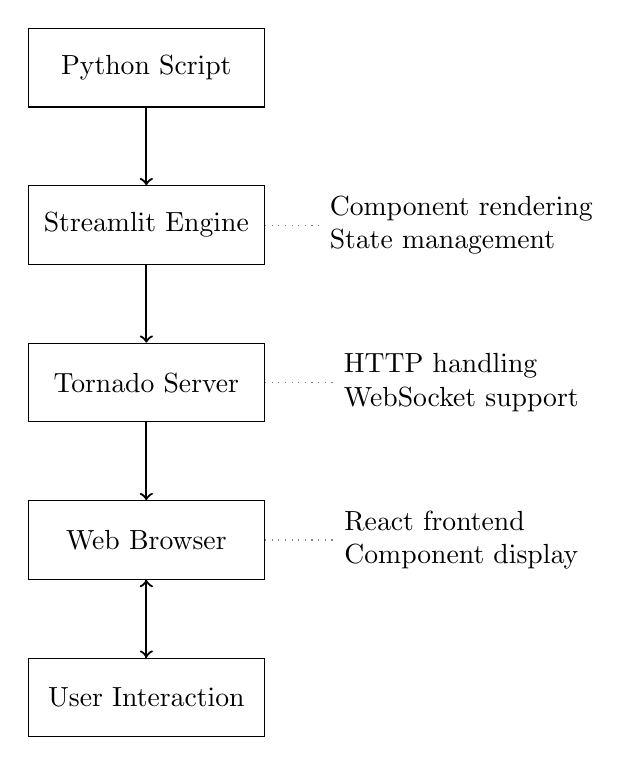
\begin{tikzpicture}[
	node distance=2cm,
	box/.style={rectangle, draw, minimum width=3cm, minimum height=1cm, align=center},
	arrow/.style={->, thick}
	]
	% Nodes
	\node[box] (script) {Python Script};
	\node[box, below of=script] (streamlit) {Streamlit Engine};
	\node[box, below of=streamlit] (tornado) {Tornado Server};
	\node[box, below of=tornado] (browser) {Web Browser};
	\node[box, below of=browser] (user) {User Interaction};
	
	% Arrows
	\draw[arrow] (script) -- (streamlit);
	\draw[arrow] (streamlit) -- (tornado);
	\draw[arrow] (tornado) -- (browser);
	\draw[arrow] (browser) -- (user);
	\draw[arrow] (user) -- (browser);
	
	% Side annotations
	\node[right of=streamlit, xshift=2cm, align=left] (engine_desc) {Component rendering\\State management};
	\node[right of=tornado, xshift=2cm, align=left] (server_desc) {HTTP handling\\WebSocket support};
	\node[right of=browser, xshift=2cm, align=left] (browser_desc) {React frontend\\Component display};
	
	% Dotted connections
	\draw[dotted, gray] (streamlit) -- (engine_desc);
	\draw[dotted, gray] (tornado) -- (server_desc);
	\draw[dotted, gray] (browser) -- (browser_desc);
\end{tikzpicture}
	\caption{Streamlit Application Architecture \cite{Streamlit:2024}}
	\label{fig:streamlit_architecture}
\end{figure}

The Streamlit architecture employs a client-server model, as illustrated in Figure \ref{fig:streamlit_architecture}. The Python script runs on the server, generating a React-based frontend that communicates via WebSocket connections. This architecture enables real-time interactivity while maintaining the simplicity of Python-only development \cite{Streamlit:2024}.

\clearpage

\section{Installation}
\label{sec:installation}

\subsection{System Requirements}
\label{subsec:system_requirements}

Streamlit requires Python 3.7 or higher and works across all major operating systems. The framework has minimal system dependencies, making installation straightforward.

\subsection{Python Package Installation}
\label{subsec:python_install}

Install Streamlit using pip:

\begin{lstlisting}[style=bashstyle, caption={Streamlit Installation}]
	# Basic installation
	pip install streamlit
	
	# Installation with common data science libraries
	pip install streamlit pandas matplotlib plotly
	
	# For development (includes testing tools)
	pip install streamlit[dev]
\end{lstlisting}

\subsection{Verification}
\label{subsec:verification}

Verify the installation by running the Streamlit hello world application:

\begin{lstlisting}[style=bashstyle, caption={Streamlit Verification}]
	streamlit hello
\end{lstlisting}

This command launches a demo application showcasing Streamlit's capabilities. The application will open in your default web browser at \texttt{http://localhost:8501}.

\subsection{Upgrading and Uninstalling}

To upgrade Streamlit to a newer version or uninstall:

\begin{lstlisting}[style=bashstyle, caption={Streamlit Maintenance}]
	# Upgrade to latest version
	pip install --upgrade streamlit
	
	# Uninstall Streamlit
	pip uninstall streamlit
\end{lstlisting}

\section{Example -- Basic Dashboard}
\label{sec:basic_example}

The following example demonstrates creating a simple data dashboard. The complete implementation with documentation is available in \texttt{BasicDashboard.py}.

\lstinputlisting[language=MyPython, caption={Basic Streamlit Dashboard}, label={lst:basicdashboard},firstline=1,lastline=50]{../Code/streamlit/BasicDashboard.py}

\noindent\textit{[The remaining code is omitted for brevity. The complete script can be found at \texttt{../Code/streamlit/BasicDashboard.py}.]}

This basic example illustrates the fundamental Streamlit workflow: creating widgets, processing data, and displaying results. The reactive nature of Streamlit automatically updates the display when users interact with widgets.

\section{Example -- Interactive Web Application}
\label{sec:interactive_example}

Advanced Streamlit applications leverage interactive widgets and state management for enhanced user experience. The integration of session state enables complex application flows and persistent data handling.


\begin{figure}[htbp]
	\centering
    % Interactive Streamlit Application Flow TikZ Diagram
% File: interactive_flow.tikz

\begin{tikzpicture}[
	node distance=1.5cm and 2cm,
	widget/.style={rectangle, draw, minimum width=2.5cm, minimum height=0.8cm, align=center, fill=blue!10},
	process/.style={ellipse, draw, minimum width=2cm, minimum height=0.8cm, align=center, fill=green!10},
	display/.style={trapezium, draw, trapezium left angle=70, trapezium right angle=110, minimum width=2cm, minimum height=0.8cm, align=center, fill=orange!10},
	arrow/.style={->, thick}
	]
	% Widgets
	\node[widget] (slider) {Slider};
	\node[widget, below of=slider] (selectbox) {Selectbox};
	\node[widget, below of=selectbox] (button) {Button};
	
	% Label for User Input under widgets
	\node[below=0.5cm of button] (inputLabel) {\textbf{User Input}};
	
	% Processing
	\node[process, right=3cm of selectbox] (compute) {Data\\Processing};
	
	% Display
\node[display, below=2cm of compute, xshift=-2.5cm] (chart) {Chart};
\node[display, right=1.5cm of chart] (metrics) {Metrics};
\node[display, right=1.5cm of metrics] (table) {Table};
	
	% Output Label under display section
	\node[below=0.3cm of metrics] {\textbf{Output Display}};
	
	% Connections
	\draw[arrow] (slider) -- (compute);
	\draw[arrow] (selectbox) -- (compute);
	\draw[arrow] (button) -- (compute);
	\draw[arrow] (compute) -- (chart);
	\draw[arrow] (compute) -- (metrics);
	\draw[arrow] (compute) -- (table);
\end{tikzpicture}
	\caption{Interactive Streamlit Application Flow}
	\label{fig:interactive_flow}
\end{figure}

The interactive application flow illustrated in Figure \ref{fig:interactive_flow} shows how user inputs trigger data processing and display updates.

\lstinputlisting[language=MyPython, caption={Interactive Streamlit Application}, label={lst:interactiveapp},firstline=1,lastline=50]{../Code/streamlit/InteractiveApp.py}

\noindent\textit{[The remaining code is omitted for brevity. The complete script can be found at \texttt{../Code/streamlit/InteractiveApp.py}.]}

\section{Example -- Machine Learning Model Deployment}
\label{sec:ml_example}

Streamlit excels at deploying machine learning models for stakeholder review and testing. The framework's simplicity enables rapid model deployment without complex infrastructure setup.

\begin{figure}[htbp]
	\centering
    % ML Model Deployment Architecture TikZ Diagram
% File: ml_deployment.tikz

\begin{tikzpicture}[
	node distance=1.5cm and 2cm,
	input/.style={rectangle, draw, minimum width=2cm, minimum height=0.8cm, align=center, fill=yellow!20},
	model/.style={rectangle, draw, minimum width=2.5cm, minimum height=1.2cm, align=center, fill=blue!20},
	output/.style={rectangle, draw, minimum width=2cm, minimum height=0.8cm, align=center, fill=green!20},
	arrow/.style={->, thick}
	]
	
	% Input section
	\node[input] (features) {Feature\\Input};
	\node[input, below=0.8cm of features] (upload) {File\\Upload};
	
	% Model
	\node[model, right=3cm of features, yshift=-0.4cm] (mlmodel) {ML Model\\Prediction};
	
	% Output section
	\node[output, right=3cm of mlmodel, yshift=0.4cm] (prediction) {Prediction\\Result};
	\node[output, below=0.8cm of prediction] (confidence) {Confidence\\Score};
	
	% Connections
	\draw[arrow] (features) -- (mlmodel);
	\draw[arrow] (upload) -- (mlmodel);
	\draw[arrow] (mlmodel) -- (prediction);
	\draw[arrow] (mlmodel) -- (confidence);
	
	% Labels
	\node[above=0.3cm of features] {\textbf{User Input}};
	\node[above=0.3cm of prediction] {\textbf{Results}};
\end{tikzpicture}
	\caption{ML Model Deployment Architecture}
	\label{fig:ml_deployment}
\end{figure}

The ML deployment architecture illustrated in Figure \ref{fig:ml_deployment} demonstrates the flow from user input to model prediction and result display.

\lstinputlisting[language=MyPython, caption={ML Model Deployment}, label={lst:mlmodel},firstline=1,lastline=50]{../Code/streamlit/MLModelApp.py}

\noindent\textit{[The remaining code is omitted for brevity. The complete script can be found at \texttt{../Code/streamlit/MLModelApp.py}.]}

\section{Performance Optimization}
\label{sec:optimization}

Optimizing Streamlit applications requires understanding caching mechanisms and state management. Proper optimization ensures responsive user experiences even with complex computations.

\subsection{Caching Strategies}
\label{subsec:caching}

Streamlit provides powerful caching decorators to improve performance:

\begin{lstlisting}[language=MyPython, caption={Caching Configuration}, label={lst:caching}]
	import streamlit as st
	
	# Cache data loading
	@st.cache_data
	def load_data():
	    return pd.read_csv("large_dataset.csv")
	
	# Cache resource initialization
	@st.cache_resource
	def load_model():
	    return joblib.load("model.pkl")
	
	# Usage
	data = load_data()
	model = load_model()
\end{lstlisting}

\subsection{Session State Management}
\label{subsec:session_state}

Managing application state for complex workflows:

\begin{lstlisting}[language=MyPython, caption={Session State Usage}, label={lst:session_state}]
	# Initialize session state
	if 'counter' not in st.session_state:
	    st.session_state.counter = 0
	
	# Update state
	if st.button("Increment"):
	    st.session_state.counter += 1
	
	st.write(f"Counter: {st.session_state.counter}")
\end{lstlisting}

\section{Error Handling and Best Practices}
\label{sec:best_practices}

Robust Streamlit applications must handle various error conditions and provide clear user feedback. Implementing proper error handling ensures a smooth user experience.

\subsection{Common Issues and Solutions}
\label{subsec:common_issues}

\begin{enumerate}
	\item \textbf{Slow Loading}: Implement caching for expensive operations
	\item \textbf{Memory Issues}: Use session state judiciously and clear unused data
	\item \textbf{User Input Validation}: Validate inputs before processing
	\item \textbf{Error Display}: Provide clear error messages to users
\end{enumerate}

\subsection{Error Handling Patterns}
\label{subsec:error_patterns}

\lstinputlisting[language=MyPython, caption={Comprehensive Error Handling with Streamlit}, label={lst:errorhandling},firstline=1,lastline=50]{../Code/streamlit/ErrorHandling.py}

\noindent\textit{[The remaining code is omitted for brevity. The complete script can be found at \texttt{../Code/streamlit/ErrorHandling.py}.]}

\section{Further Reading}
\label{sec:further_reading}

To deepen understanding of Streamlit and its applications, consider these resources:

\subsection{Official Documentation}
\begin{itemize}
	\item \textbf{Streamlit Documentation}: \url{https://docs.streamlit.io/}
	\item \textbf{Streamlit GitHub Repository}: Official source code repository \cite{Streamlit:2024}
	\item \textbf{Streamlit Gallery}: \url{https://streamlit.io/gallery}
	\item \textbf{Streamlit Community Forum}: \url{https://discuss.streamlit.io/}
	\item \textbf{Streamlit Components}: \url{https://towardsdatascience.com/how-to-structure-and-organise-a-streamlit-app-e66b65ece369/}
\end{itemize}

\subsection{Tutorials and Guides}
\begin{itemize}
	\item \href{https://blog.streamlit.io/}{Official Streamlit Blog}
	\item \href{https://streamlit.io/cloud}{Streamlit Cloud Deployment Guide}
	\item \href{https://towardsdatascience.com/beginners-guide-to-streamlit-for-deploying-your-data-science-projects-9c9fce488831/}{Streamlit 101 Tutorial} \cite{Towards:2023}
\end{itemize}

\section{Conclusion}
\label{sec:conclusion}

Streamlit provides a powerful and accessible solution for creating data-driven web applications with pure Python. From simple dashboards to complex machine learning deployments, Streamlit's intuitive API and reactive model make it an indispensable tool for data scientists and developers. The examples and techniques presented in this chapter provide a foundation for building robust interactive applications, while the architectural understanding enables optimization for specific use cases.\\

Future developments in Streamlit focus on enhanced component libraries, improved performance optimization, and expanded deployment options \cite{Chen:2023}. As the data science field continues to evolve, Streamlit remains at the forefront of democratizing web application development, empowering data professionals worldwide to share their insights through interactive and engaging applications.